
\label{sec:expt}

In this section we report our results and findings of static and dynamic instruction count, performance, power, and energy. 

\subsection{Instruction Count}
Figure~\ref{fig:static} shows the static icount obtained from QEMU. As seen in the figure, on average 32bit and 64bit ARM are about 15\% more dense than that of in MIPS and RISCV. Mibench applications have on average 5k instruction that are executed at least once. Figure~\ref{fig:dynamic} shows the dynamic icount obtained from QEMU. Unlike static icount, dynamic icount can be quite different from one application to another for different ISAs. However, on average MIPS, ARM, and RISCV have almost same dynamic icount. 

\begin{figure*}[htb]
	\centering
	%\footnotesize
	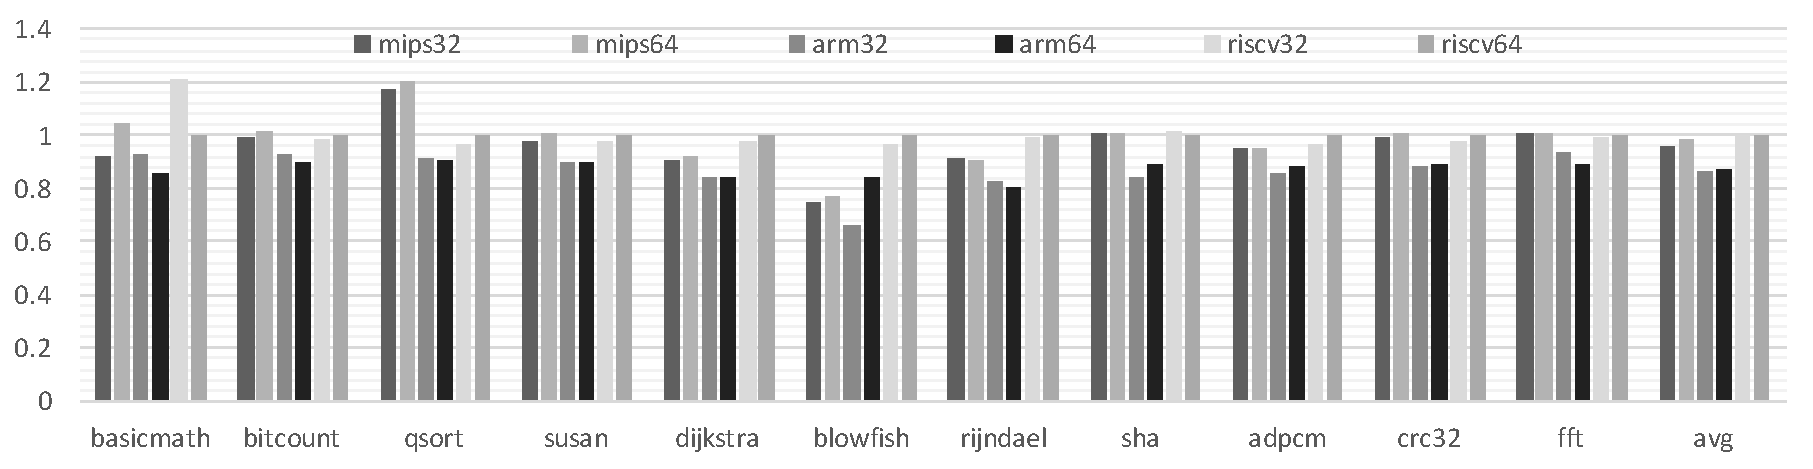
\includegraphics[width=1.9\columnwidth]{figures/static.pdf}
	\caption{Static Instruction Count for MiBench applications using QEMU. Results are normalized w.r.t. RISCV64. The average number of static instructions is about 5000 for these benchmarks.}
	\label{fig:static}
	%\vspace{-1em}
\end{figure*} 

\begin{figure}[htb]
	\centering
	%\footnotesize
	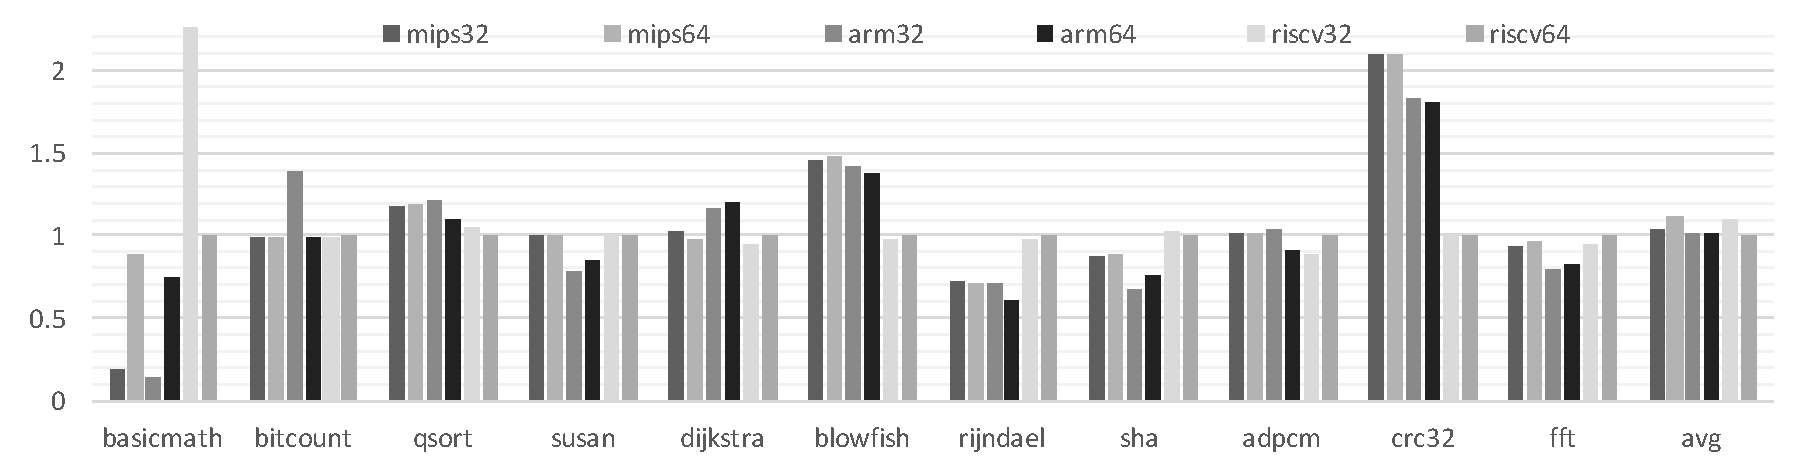
\includegraphics[width=1\columnwidth]{figures/dynamic.pdf}
	\caption{Dynamic Instruction Count for MiBench applications using QEMU. Results are normalized w.r.t. RISCV64. The average number of dynamic instructions for these benchmarks is about 450 million.}
	\label{fig:dynamic}
	\vspace{-1em}
\end{figure} 

\noindent \textbf{Key Findings}: 1- Mixed/Combined instructions (e.g. add+shift, mult+add, etc.) and three operand/three-way comparison in ARM could result in significant dynamic and static icount reduction. A possible and interesting extension to RISCV could be adding this sort of instructions to the base ISA (RV-G) for high-performance scenarios. An example is shown in Figure~\ref{fig:code}, where a same function is shown for ARM and RISCV ISAs. As seen in this example, ``ldr'' instruction in ARM with embedded ``lsl'' instruction inside it, has saved one instruction. Further ``cmn'' (compare and add), also saved two extra instructions in ARM. We found that there are many examples such as this where more complex instructions in ARM could save more space, however, we will later show that this complexity comes with more power consumption. 

\noindent 2- RISCV compiler tends to use many load/store to stack/register files which could be saved by using extra registers. A better compiler is needed to improve register utilizations to remove unnecessary load/store register instruction and improve code density in RISCV. Moreover, ARM has a more intelligent compiler where it can unroll and/or saves some instructions in a loop body. This could in turn be very beneficial when the loop is hot. 

\noindent 3- Checking some of the outliers we found that runtime libraries could play an important role in dynamic behavior of the system for these applications, and interestingly there were cases that some of glibc/gnu libraries were implemented differently in RISCV. Overall, introduction of RISCV provides a unique opportunity to rethink and re-evaluate many existing runtime libraries which could lead to non-negligible performance/power efficiency improvements. 

\noindent 4- RISCV has a more straightforward way to handle branches (compared to ARM) which could save many cycles in hot loops in some cases. 
\\




\begin{figure}[]
	\centering
	%\footnotesize
	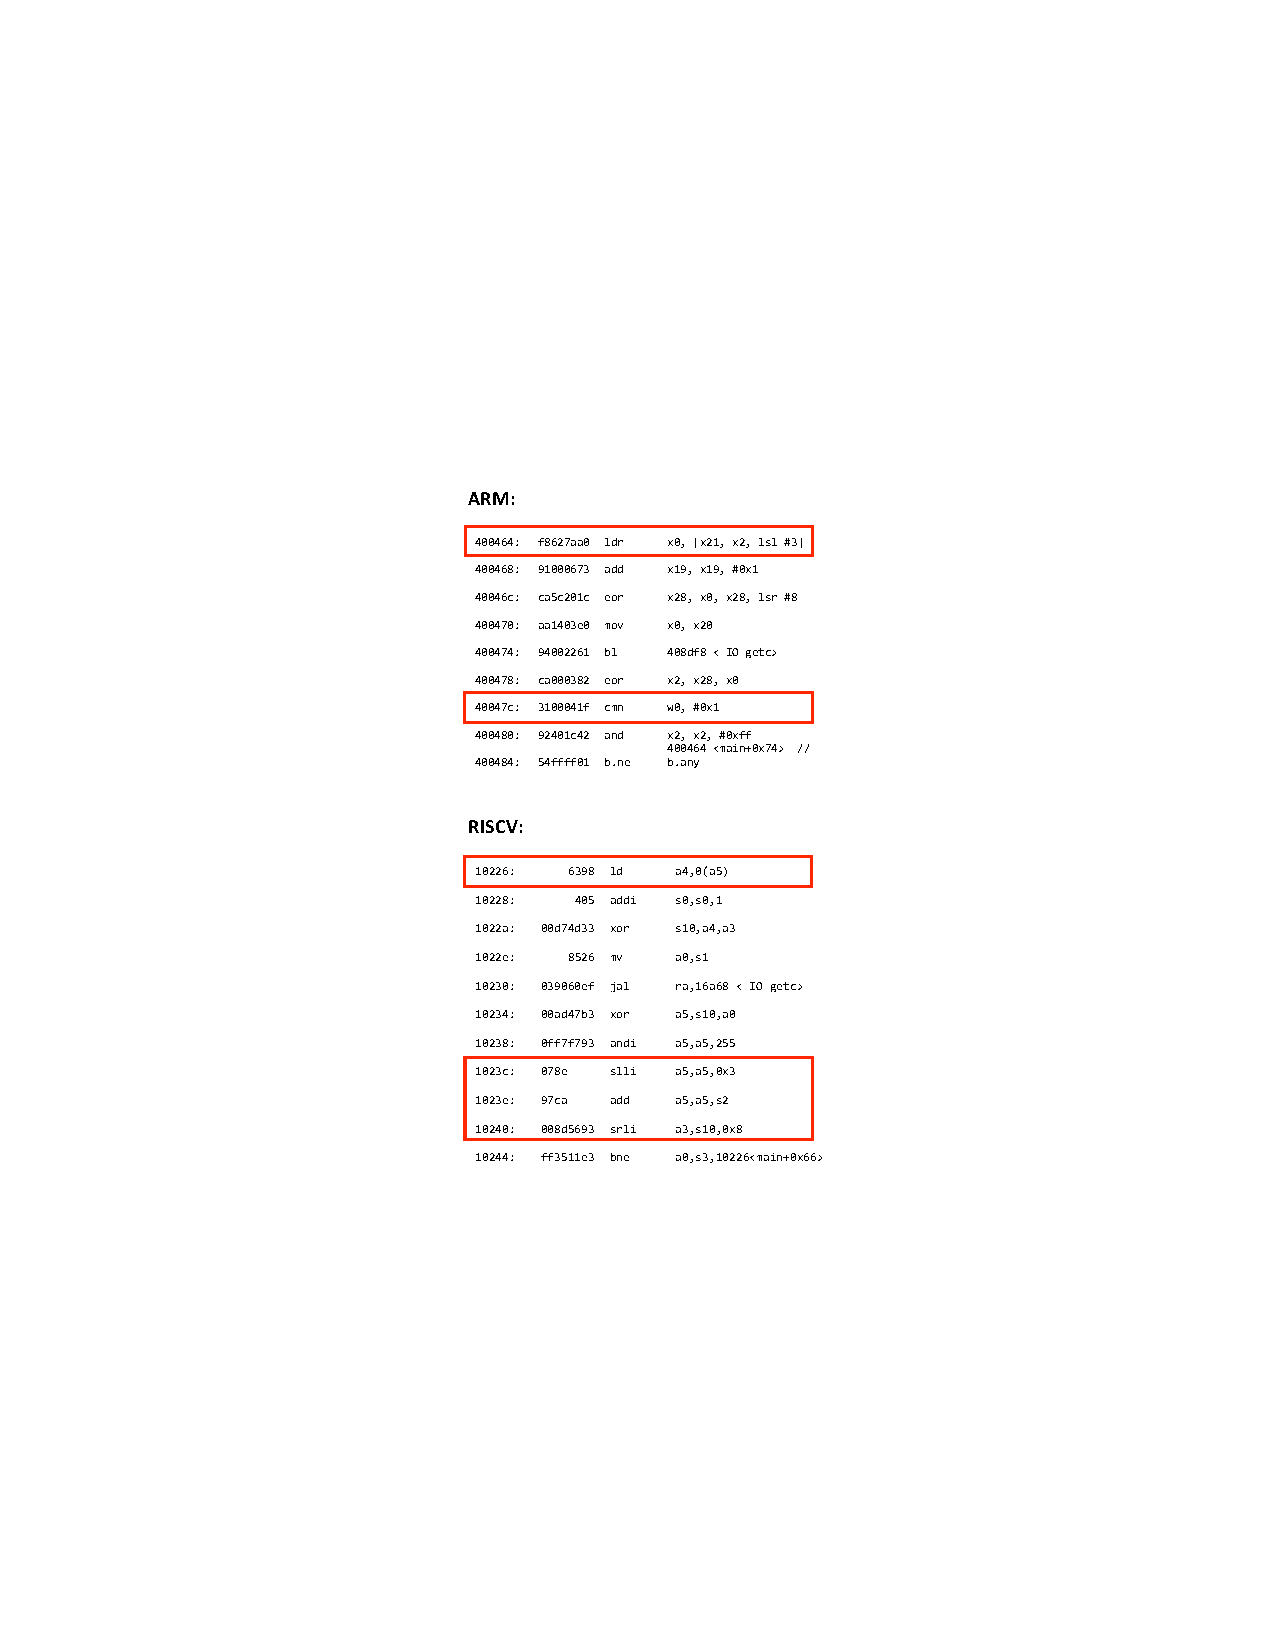
\includegraphics[width=0.8\columnwidth]{figures/code.pdf}
	\caption{A code snippet in assembly showing a same function from Mibench benchmark suite for ARM-64 and RISCV-64 ISAs. Differences shown in rectangles.}
	\label{fig:code}
	%\vspace{-1em}
\end{figure} 

\begin{figure*}[htb]
	\centering
	%\footnotesize
	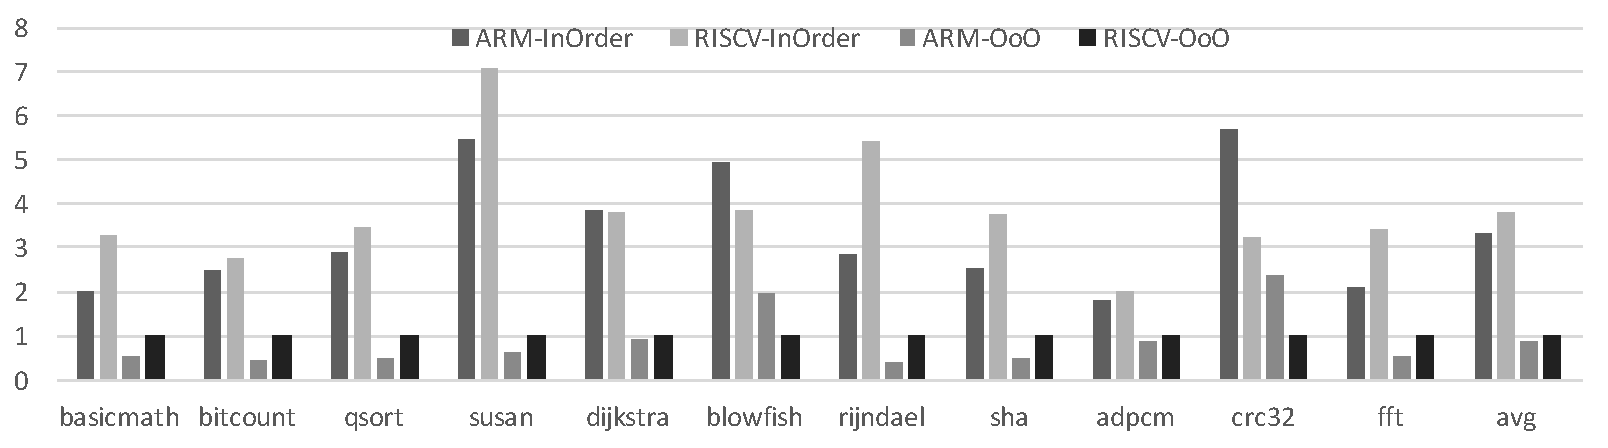
\includegraphics[width=1.9\columnwidth]{figures/cyc.pdf}
	\caption{Total number of cycles for RISCV and ARM cores (lower is better). Results are normalized w.r.t. RISCV-Out-of-Order core. The average number of cycles is about 300 million for OoO cores and 1 billion for In-Order cores.}
	\label{fig:totCyc}
	%\vspace{-1em}
\end{figure*} 

\begin{figure}[]
	\centering
	%\footnotesize
	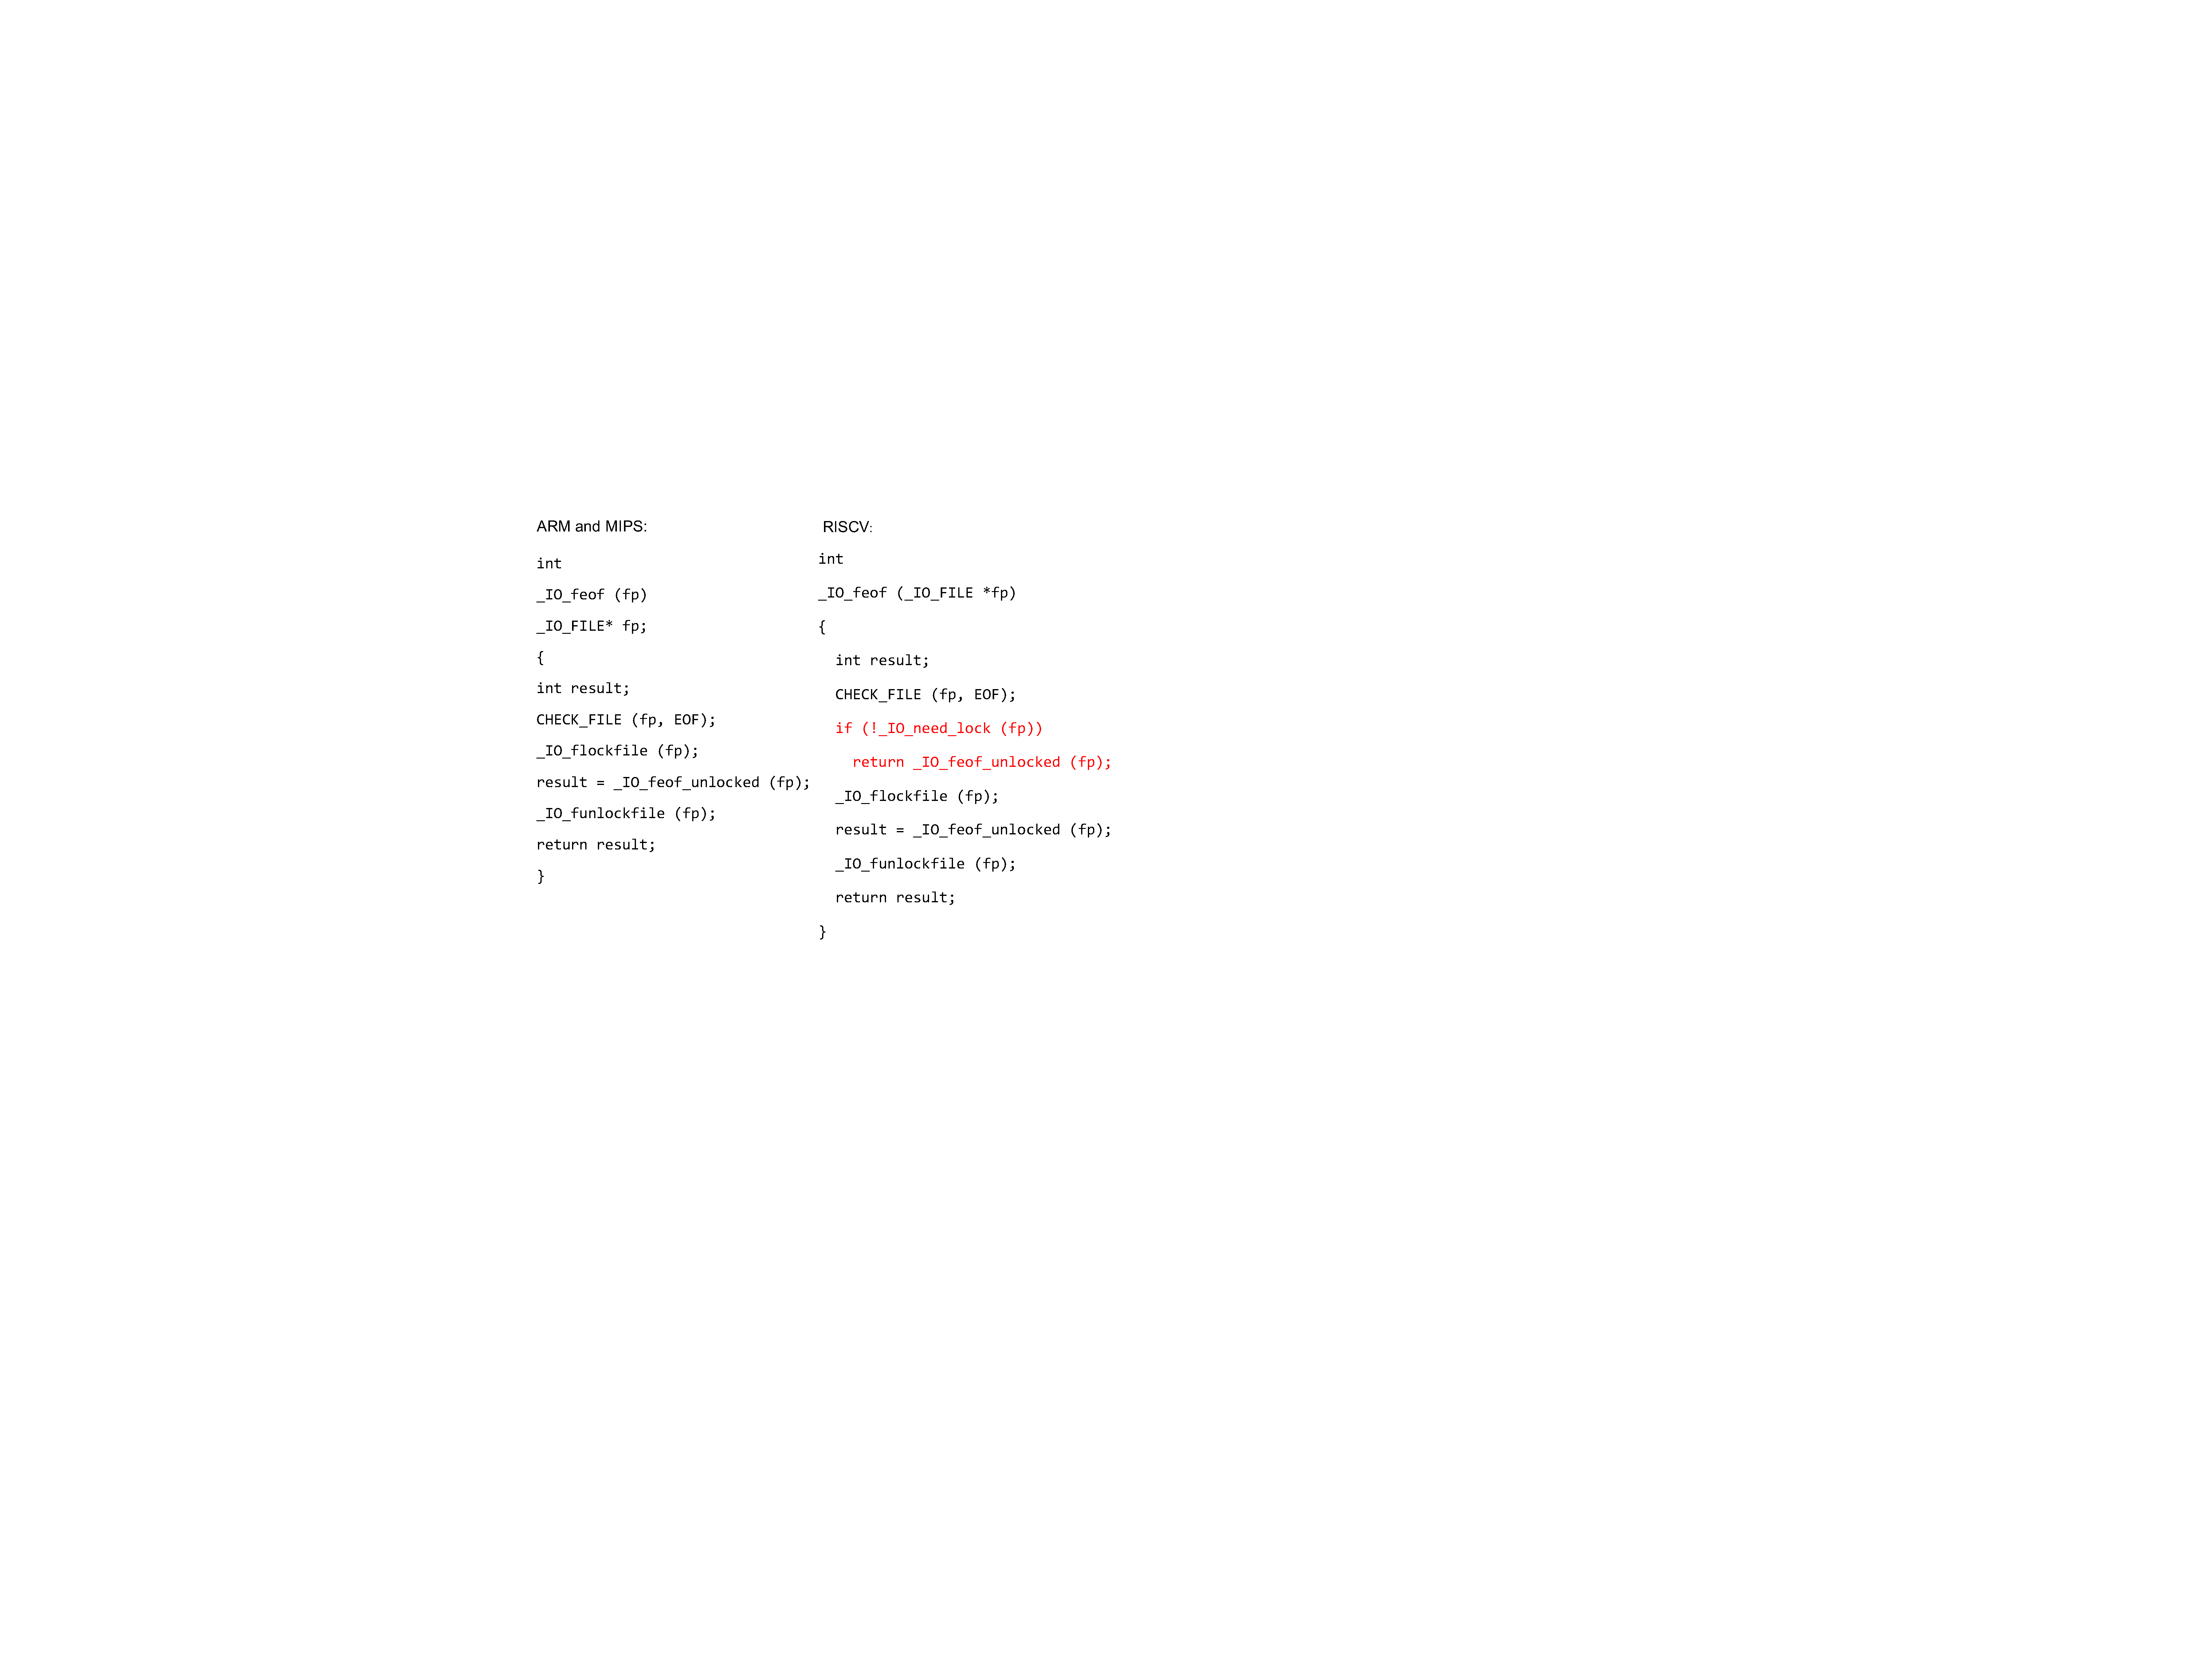
\includegraphics[width=1\columnwidth]{figures/libc.pdf}
	\caption{A code snippet in C showing a same IO subroutine implemented in glibc for ARM, MIPS, and RISCV. Differences shown in red.}
	\label{fig:libc}
	\vspace{-1em}
\end{figure} 


\noindent \textbf{Outliers}: Apart from better density (in static icount) in ARM due to combined/complex instructions, for ``basicmath'', the main reason for different dynamic icount among ISAs is due to the way \textit{long double} data type is handled (by default) in different compilers. Some used native floating point instructions for mult/div this data type, and the some used software libraries (e.g. \textit{gnu mulf3}). For ``crc32'' and ``blowfish'' the main reason for significantly lower icount in RISCV is the way an IO library (part of glibc) is implemented where in RISCV the code first checked whether an atomic lock is needed (shown in Figure~\ref{fig:libc}). 


static icount for qsort on MIPS is significantly higher. The main reason for that is due to the way a hot loop in a function called \textsc{msort\_with\_temp} (part of glibc library for quicksort) is implemented in MIPS where a few extra instructions are used for MIPS. Interestingly, we find that this function is implemented slightly different among different toolchains. 

\begin{figure}[]
	\centering
	%\footnotesize
	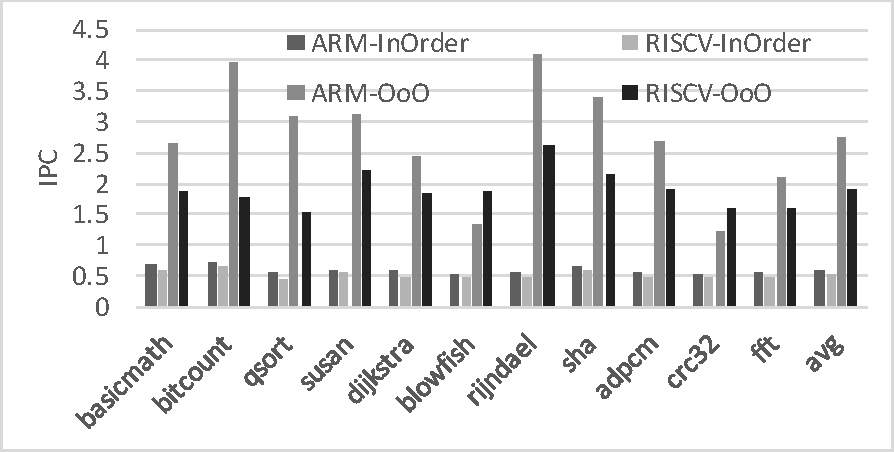
\includegraphics[width=1\columnwidth]{figures/ipc.pdf}
	\caption{Instruction per Cycle (IPC) for RISCV and ARM out-of-order cores.}
	\label{fig:ipc}
	\vspace{-1em}
\end{figure} 


\subsection{Performance}
Figure~\ref{fig:totCyc} shows the total number of cycles (from beginning to the end of program using same inputs) for 2 in-order and 2 out-of-order cores simulated in gem5. As seen in the figure, overall ARM in-order and out-of-order cores are faster by 5\% and 13\% over RISCV cores. To further investigate the performance, Figure~\ref{fig:ipc} shows the IPC for RISCV and ARM cores. As seen in this figure, ARM in-order and out-of-order cores have better IPC than RISCV cores by 13\% and 42\% respectively. Followings show our key findings about IPC and performance:

\noindent \textbf{Key Findings}: 1- Looking at different statistics in gem5, we found that the main reason for lower performance in RISCV is that it uses significantly larger indirect jumps and function calls (more than 100x!). This, in turn, leads to a poor branch prediction accuracy and results in a large number of wasted/squashed cycles due to branch mispredictions. We didn't find anything fundamentally wrong with RISCV ISA that could cause this and we believe this problem is mainly due to the RISCV compiler performance. A possible solution to this problem is either fixing the RISCV compiler to reduce the number of indirect branches and improve the inlining or improve the branch predictor accuracy on indirect branches. 

\noindent 2- Apart from indirect jumps, branch predictor accuracy, and number of function calls, almost all other micro-architectural statistics (e.g. MPKI, stalls, etc.) are the same for RISCV and ARM processors.

\noindent 3- Instruction mix is ISA-independent. Both ISAs have almost the same ALU, LOAD, STORE, and BR instruction distribution. 

\noindent 4- Cycle Count for In-order processors closely follows the dynamic icount thus it can directly be benefited from better compiler and/or custom instructions. \\

\noindent \textbf{Outliers}: ``crc32'' and ``blowfish'' have poor performance on ARM processors. Looking into the statistics, we found that this poor performance is mainly due to a large serialized atomic loads to main memory (mainly because of activities in \textsc{\_IO\_flockfile ()} shown in Figure~\ref{fig:libc}) which causes lots of stall cycles and pipeline underutilization in ARM cores (especially for OoO core). 

\subsection{Power and Performance}






